Pierwszym przeprowadzonym testem było sprawdzenie wydajności układu podczas procesu chłodzenia obiektu.
\begin{figure}[H]
	\centering
	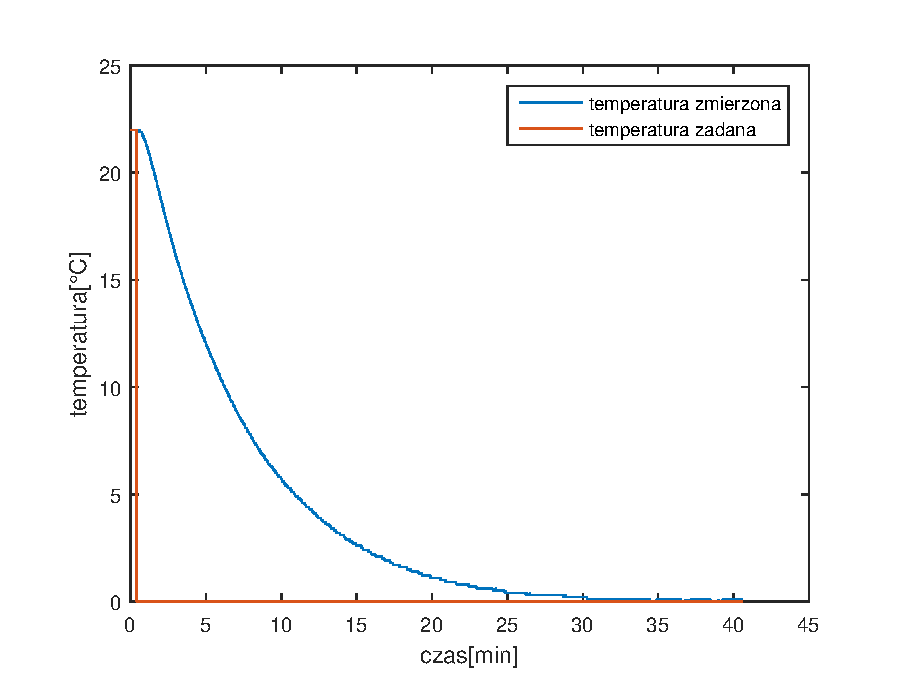
\includegraphics[scale=0.75]{test_chlodzenia.eps}
	\caption{Test wydajności układu regulacji temperatury}
	\label{fig:chlodzenie}
\end{figure}
Podczas całego procesu ogniwo pracowało z pełną mocą. Proces rozpoczął się od ustabilizowania temperatury na 22 stopniach Celsjusza. Następnie, na sterownik ogniwa zadano sygnał PWM o maksymalnej częstotliwości. Na rysunku 7.1 można zaobserwować, że obiekt został bardzo szybko schłodzony do temperatury poniżej 10 stopni. Granicą wydajności okazała się temperatura zbliżona do zera, na której odczyt ustabilizował się po 35 minutach. Osiągnięta wartość okazała się znacznie niższa niż przewidywano.

Ze względu na duże temperatury osiągane przez ogniwo (do ponad $100^{\circ} C$) podczas ogrzewania zdecydowano, że test maksymalnej osiągniętej temperatury w obiekcie nie zostanie przeprowadzony.
\section{Regulator histerezowy}
W pierwszej kolejności przetestowano najbardziej podstawowy regulator- histerezowy. Otrzymane wyniki są zbliżone do temperatury zadanej. Regulator histerezowy charakteryzuje się dużą stabilnością przebiegu, którą można zaobserwować na rysunku ~\ref{fig:hist18} i ~\ref{fig:hist26}.
\begin{figure}[H]
	\centering
	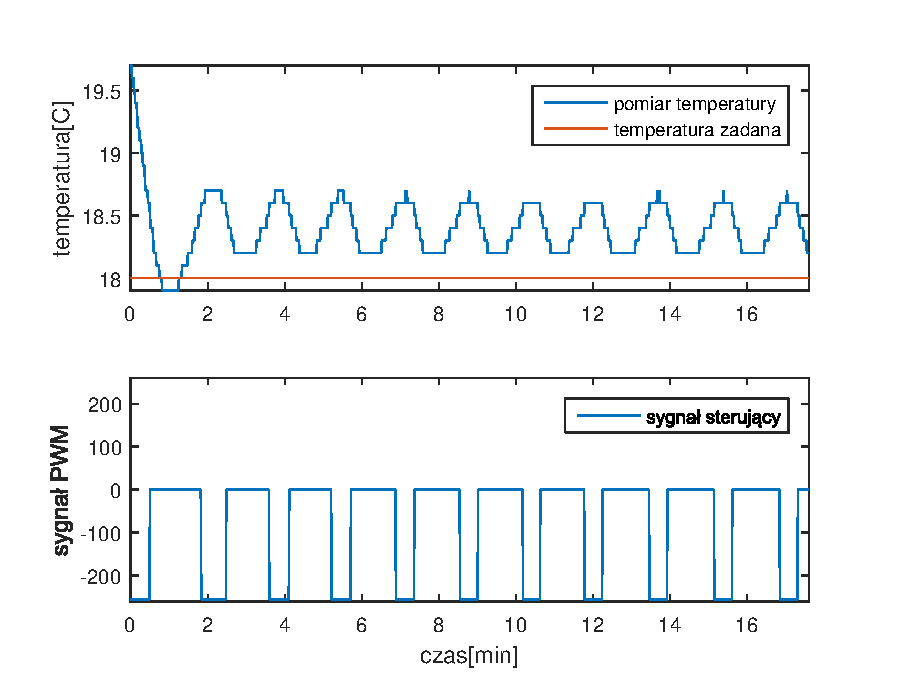
\includegraphics[scale=0.8]{hist18.eps}
	\caption{Regulator histerezowy. Histereza 0.5 stopnia.}
	\label{fig:hist18}
\end{figure}

\begin{figure}[H]
	\centering
	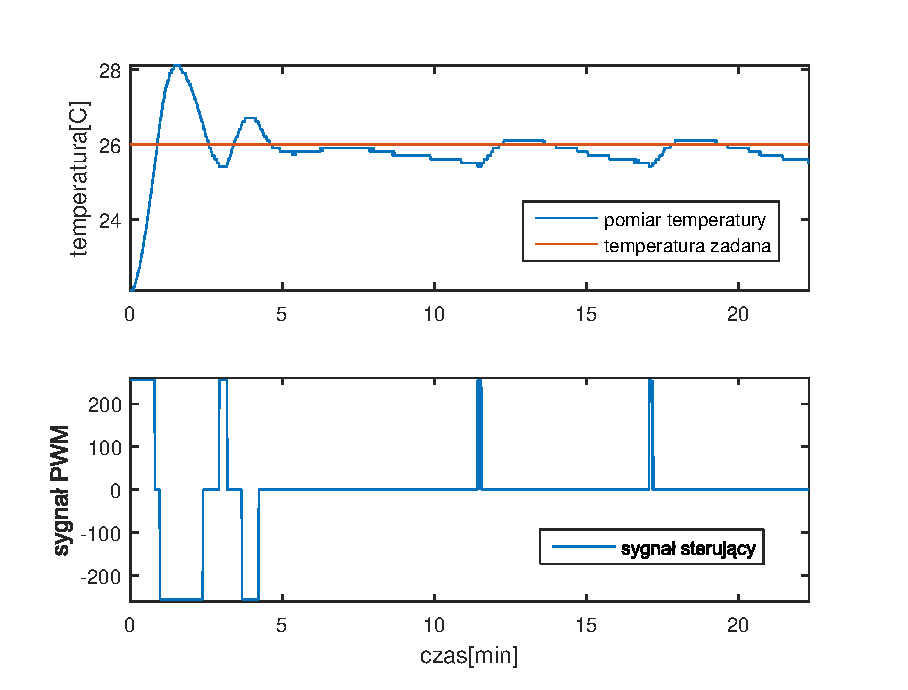
\includegraphics[scale=0.8]{hist26.eps}
	\caption{Regulator histerezowy. Histereza 0.5 stopnia.}
	\label{fig:hist26}
\end{figure}
\newpage
\section{Regulator PID}
Test regulatora PID został podzielony na etapy, w których przetestowano wpływ nastaw regulatora na działanie każdego z członów. Podczas testów członu całkującego i różniczkującego wykorzystano również człon proporcjonalny.

\subsection{P}
\begin{figure}[H]
	\centering
	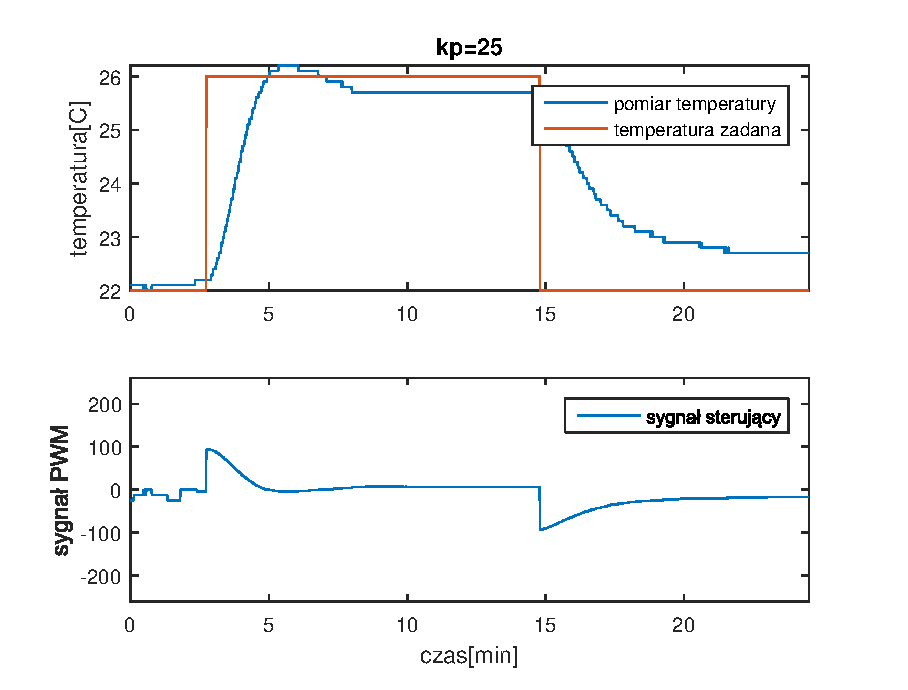
\includegraphics[scale=0.9]{26kp25.eps}
	\caption{Regulator P, kp=25}
	\label{fig:kp25}
\end{figure}
Na rysunku ~\ref{fig:kp25} można zaobserwować, że dla niskiej wartości wzmocnienia członu proporcjonalnego,temperatura szybko stabilizuje się, ale na poziomie niższym od zadanego. Przy wartości kp=25, regulator nie jest w stanie osiągnąć zadanej temperatury podczas procesu chłodzenia.
\newpage
\begin{figure}[H]
	\centering
	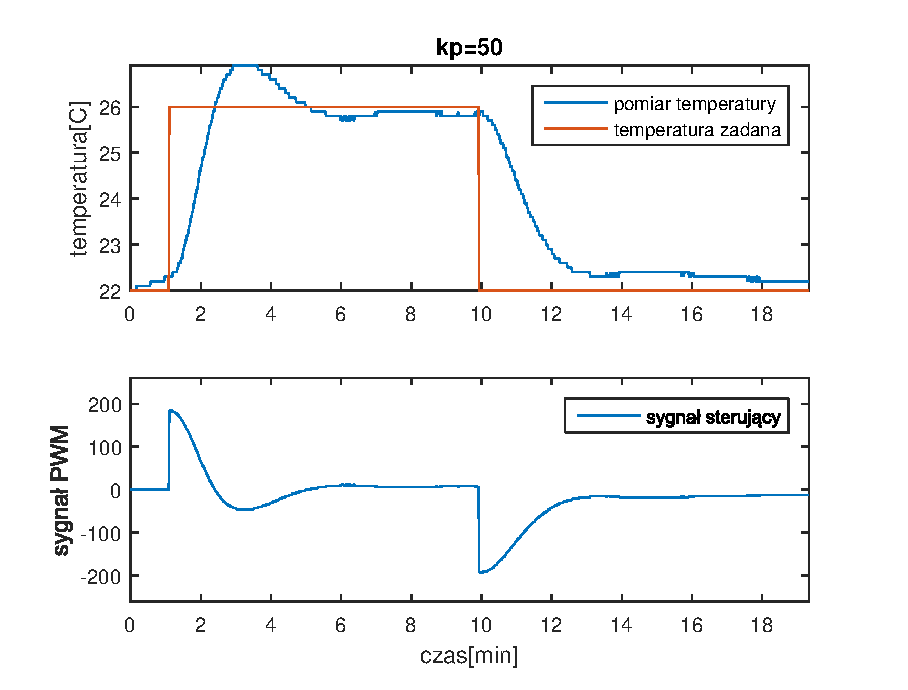
\includegraphics[scale=0.9]{26kp50.eps}
	\caption{Regulator P, kp=50}
	\label{fig:kp50}
\end{figure}
\begin{figure}[H]
	\centering
	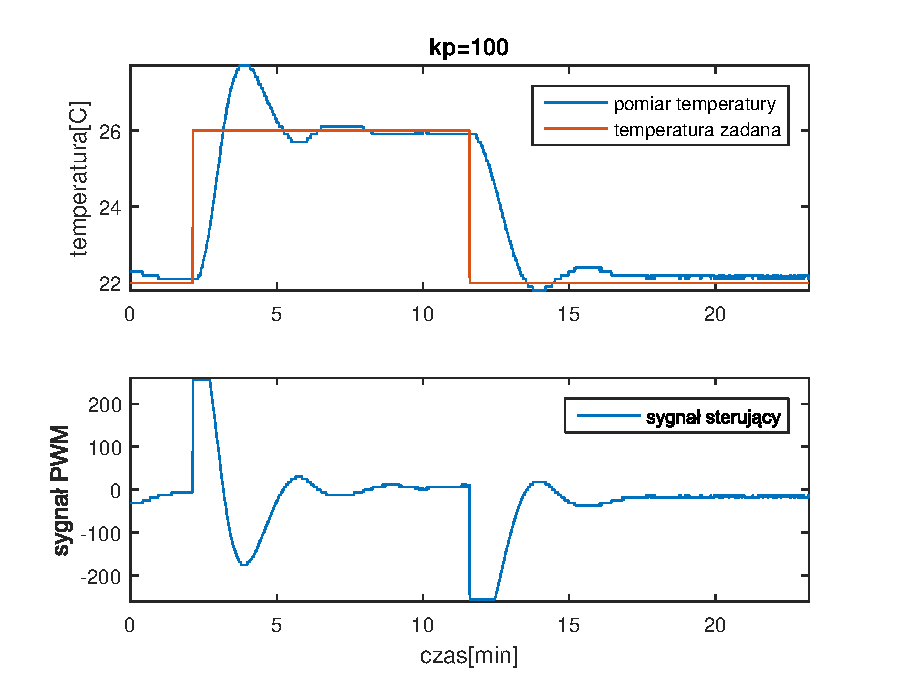
\includegraphics[scale=0.9]{26kp100.eps}
	\caption{Regulator P, kp=100}
\end{figure}
\begin{figure}[H]
	\centering
	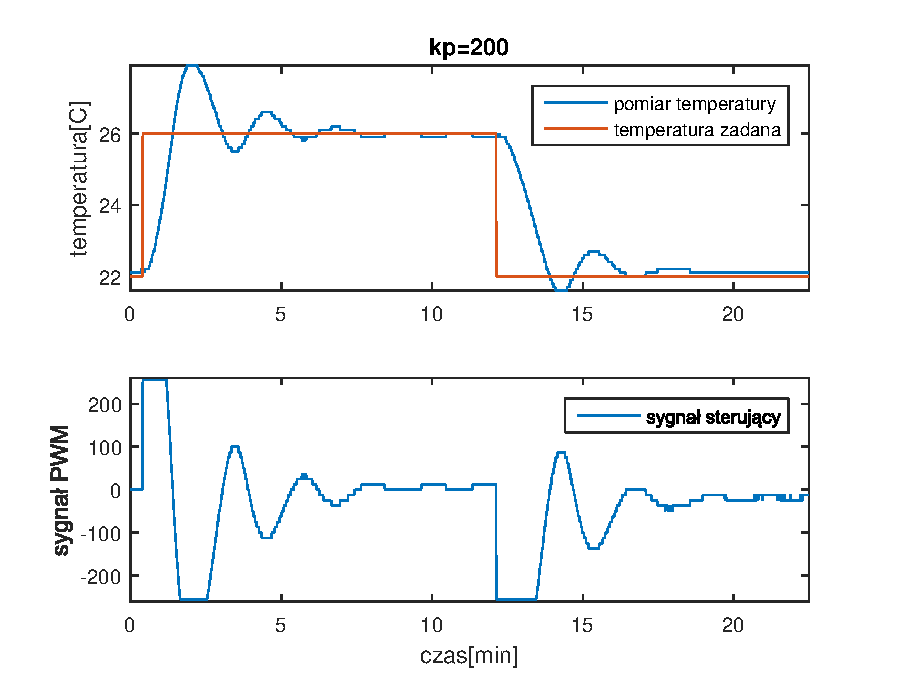
\includegraphics[scale=0.9]{26kp200.eps}
	\caption{Regulator P, kp=200}
	\label{fig:kp200}
\end{figure}
Po zwiększeniu wzmocnienia do 50, na rysunku ~\ref{fig:kp50} można zaobserwować nieznaczną poprawę czasu narastania, ale pojawiły się niedogodności w postaci przeregulowania na poziomie $1^{\circ} C$. Tym razem temperatura  ustaliła się bliżej wartości zadanej. Proces chłodzenia również przebiegł znacznie sprawniej.

Kolejne dwukrotne zwiększenia nastawy regulatora spowodowało znaczne skrócenie czasu narastania, ale wydłużyło czas regulacji. Przeregulowania przekroczyły wartość $2^{\circ} C$. Na charakterystyce pojawiły się powoli tłumione oscylacje temperatury.
\newpage

\subsection{PI}

\begin{figure}[H]
	\centering
	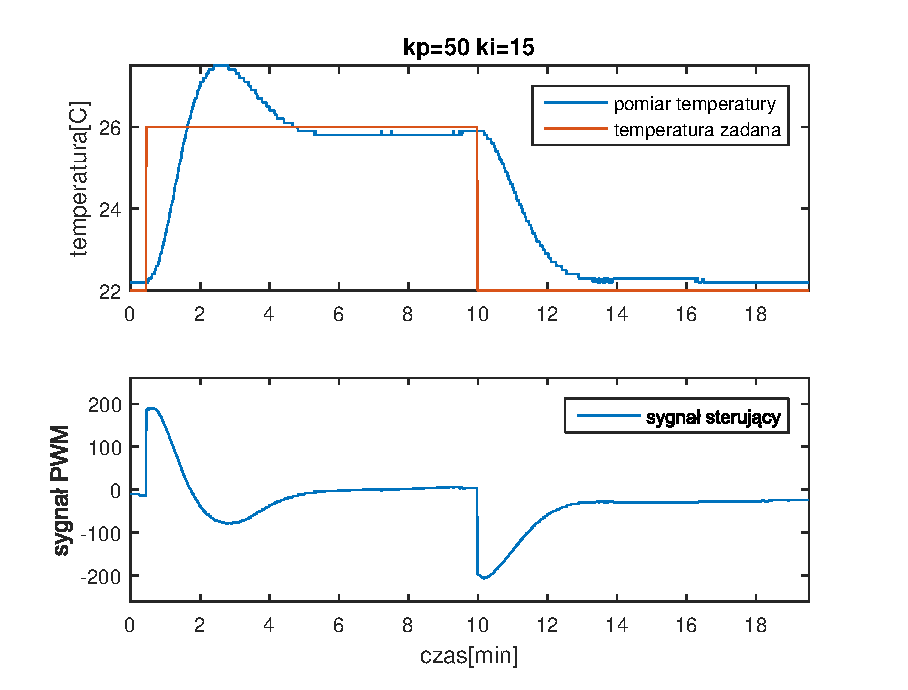
\includegraphics[scale=0.9]{26kp50ki15.eps}
	\caption{Regulator PI, kp=50 ki=15}
	\label{fig:ki15}
\end{figure}
\begin{figure}[H]
	\centering
	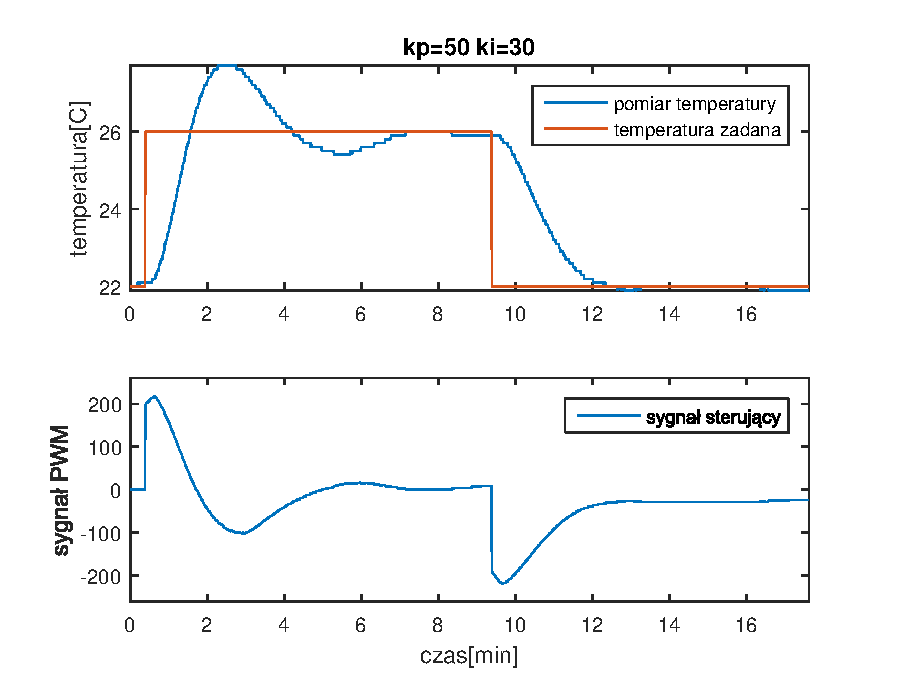
\includegraphics[scale=0.9]{26kp50ki30.eps}
	\caption{Regulator PI, kp=50 ki=30}
	\label{fig:ki30}
\end{figure}

Wprowadzenie członu całkującego o małej wartości (rysunek ~\ref{fig:ki15}), wyraźnie skróciło czas narastania. Dodatkowym skutkiem okazało się przybliżenie wartości otrzymanej do oczekiwanej, również podczas chłodzenia. Znacznym problemem wykorzystanych nastaw jest narastanie członu całkującego, który później powoduje powstanie znacznych przeregulowań.

Podczas kolejnego testu, zwiększono wzmocnienie całkujące do 30. Przeregulowanie nieznacznie wzrosło. Czas regulacji wydłużył się z powodu pojedynczej oscylacji, widocznej na rysunku ~\ref{fig:ki30}. Temperaturę można uznać za prawidłowo wyregulowaną. Po ustaleniu się, odstępstwa od wartości zadanej wynosiły jedynie 0.1 stopnia, co jest wartością bardzo zadowalającą dla pomiaru wykonywanego z dokładnością +/- 0.5 stopnia.

Kolejne zwiększenie nastawy \textit{ki} przedstawione na rysunku ~\ref{fig:ki60}, nie przyniosło pozytywnych efektów. Podczas ogrzewania zaobserwowano wielokrotne przeregulowania. Oscylacje pojawiły się również podczas ochładzania obiektu. Czas narastania skrócił się, a czas regulacji znacznie wydłużył.

\begin{figure}[H]
	\centering
	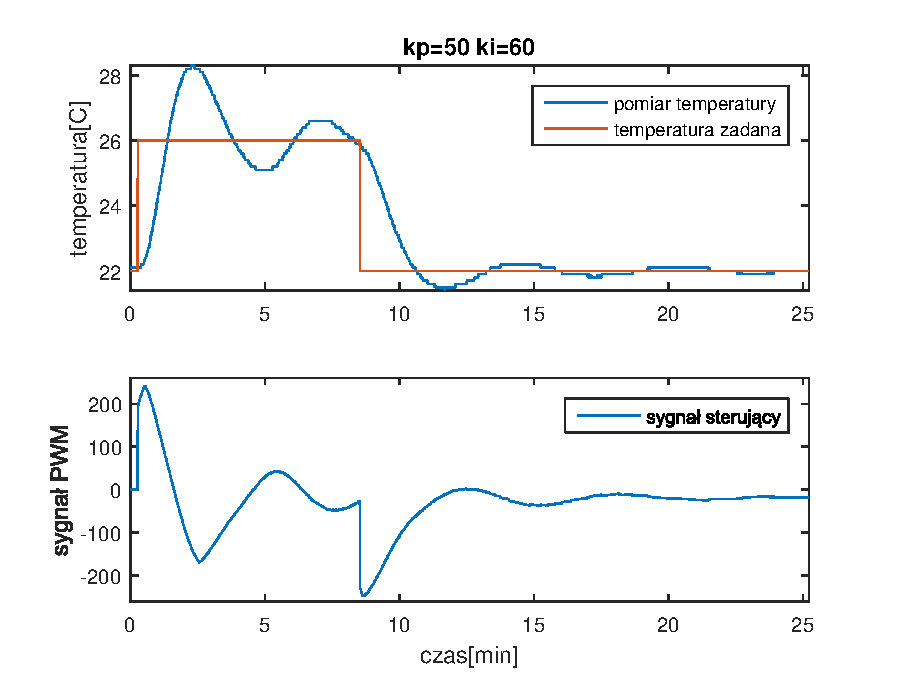
\includegraphics[scale=0.9]{26kp50ki60.eps}
	\caption{Regulator PI, kp=50 ki=60}
	\label{fig:ki60}
\end{figure}

Najkorzystniejszym rozwiązaniem okazała się pośrednia wartość wzmocnienia członu całkującego. Dla wartości zbyt małej, efekty włączenia członu I są praktycznie niewidoczne. Wprowadzenie dużego wzmocnienia zmniejsza ostateczny błąd regulacji, kosztem pojawienia się licznych oscylacji i znacznego wydłużenia procesu regulacji.
\newpage

\subsection{PD}
Pierwszy test członu różniczkującego przebiegł zgodnie z oczekiwaniami. Na rysunku ~\ref{fig:kp200} można zaobserwować, że wzmocnienie \textit{kp}=200 spowodowało pojawienie się dużego przeregulowania oraz oscylacji. W przykładzie z rysunku ~\ref{fig:kd20}, wartość wzmocnienia proporcjonalnego zwiększono o kolejne 50 jednostek. Po dodaniu członu D, przebieg temperatury został spłaszczony i ustalił się szybciej niż dla samego członu P.
\begin{figure}[H]
	\centering
	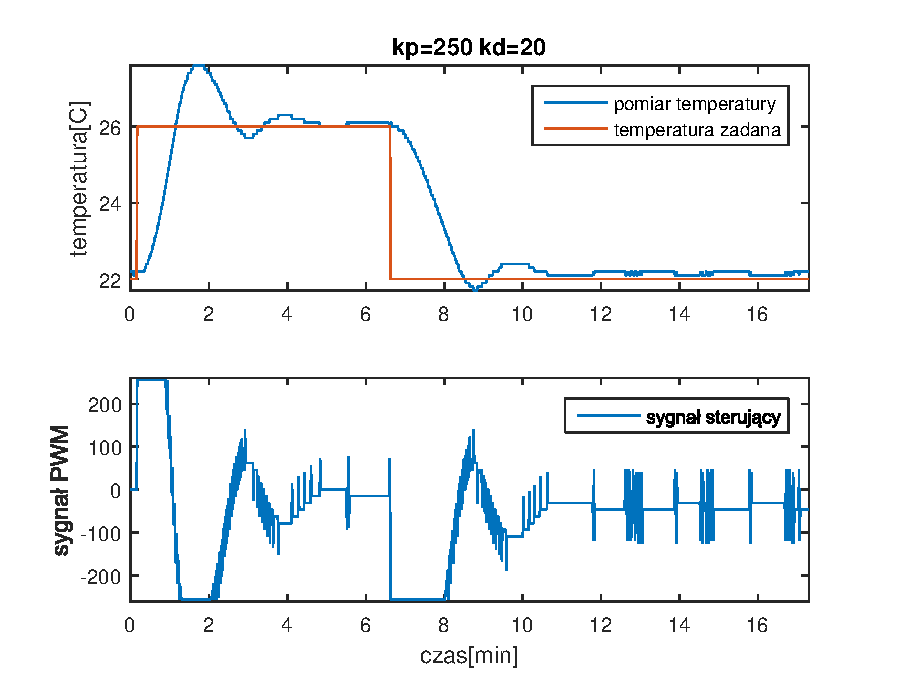
\includegraphics[scale=0.9]{26kp250kd20.eps}
	\caption{Regulator PD, kp=250 kd=20}
	\label{fig:kd20}
\end{figure}
Kolejne zwiększenia wartości nastawy \textit{kd}, spowodowały znaczne zmniejszenie wartości przeregulowania oraz prawie całkowicie zniwelowały występowanie oscylacji.

Po ustawieniu parametru na 80 jednostek, przeregulowanie zostało ograniczone z  2 stopni Celsjusza do około 0.5 stopnia. Niestety, przy tak dużym wzmocnieniu członu D, temperatura ustala się powyżej wartości zadanej.
\newpage
\begin{figure}[H]
	\centering
	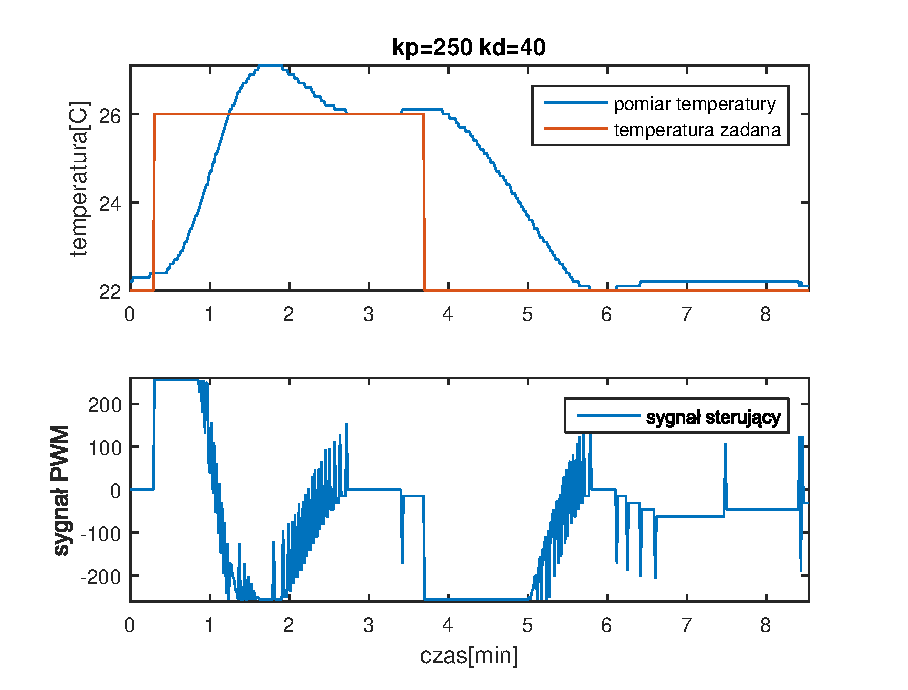
\includegraphics[scale=0.9]{26kp250kd40.eps}
	\caption{Regulator PD, kp=250 kd=40}
\end{figure}
\begin{figure}[H]
	\centering
	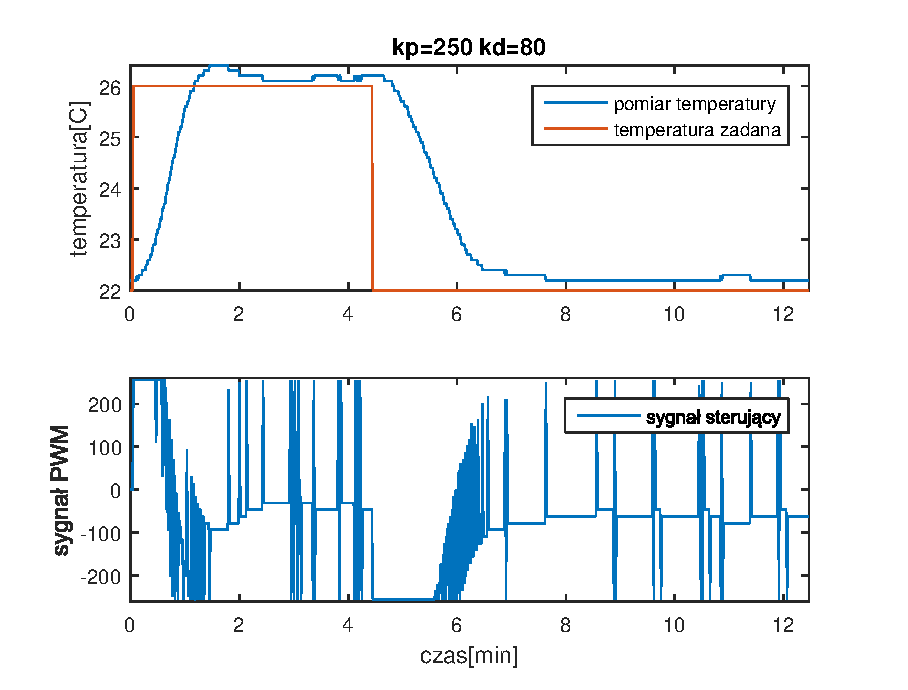
\includegraphics[scale=0.9]{26kp250kd80.eps}
	\caption{Regulator PD, kp=250 kd=80}
\end{figure}

\subsection{PID}
W celu zniwelowania niekorzystnych efektów używania członu I oraz D, należy wykorzystać regulator PID, który po dobraniu odpowiednich nastaw powinien pozwolić na ograniczenie przeregulowania oraz oscylacji, bez pogorszenia czasu narastania i regulacji temperatury.

Nastawy regulatora zostały dobrane ręcznie, po wykonaniu licznych prób i testów działania regulatora. Duża wartość parametru \textit{kp} i \textit{ki} pozwoliła na zmniejszenie czasu narastania poniżej 2 minut. Dzięki członowi \textit{D}, zmniejszono wartość przeregulowania. Odstępstwa temperatury zmierzonej od zadanej na poziomie +/-0.1 stopnia, uznano za bardzo dobry wynik.

Poniżej przedstawiono wybrane testy dla temperatur z przedziału od 18 do 30 stopni Celsjusza. Optymalne nastawy regulatora to: \textit{kp}=250, \textit{ki}=62, \textit{kd}=80.
%\begin{itemize}
%\item \textit{kp}=250,
%\item \textit{ki}=62,
%\item \textit{kd}=80.
%\end{itemize}
Podczas chłodzenia obiektu przeregulowanie nie występuje, a temperatura zostaje bardzo szybko zbliżona do zadanej. W kolejnych minutach temperatura stopniowo zbliża się do zadanej wartości. Pojawiające się na przebiegu sygnału sterującego \textit{szpilki}, są wynikiem działania części różniczkującej regulatora, w ten sposób hamowane jest narastanie temperatury podczas zbliżania się do wartości zadanej.
\begin{figure}[H]
	\centering
	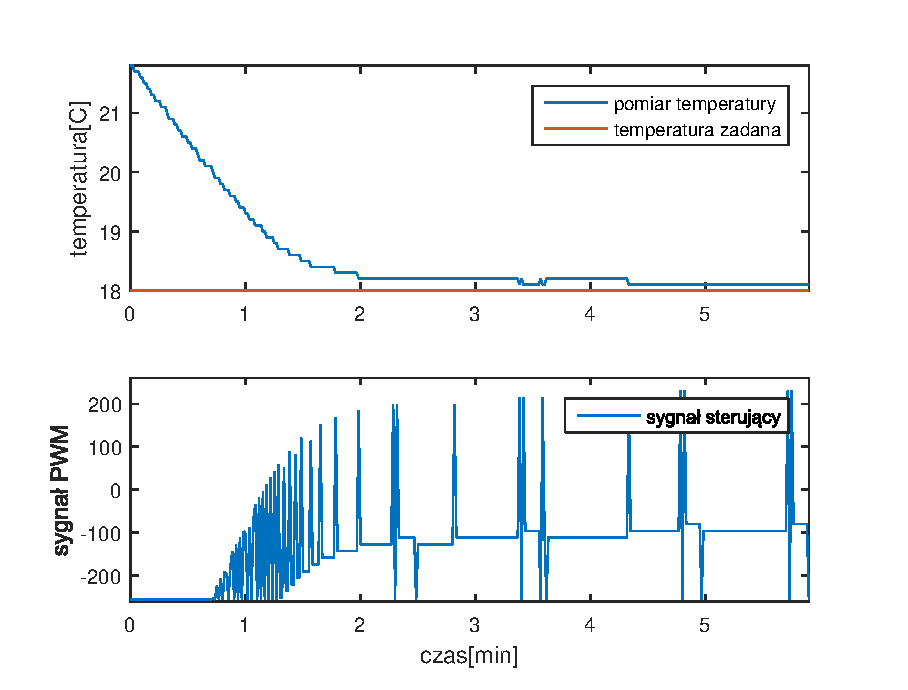
\includegraphics[scale=0.9]{pid18.eps}
	\caption{Regulacja dla $18^{\circ} C$}
	\label{fig:pid18}
\end{figure}
Na wykresie ~\ref{fig:pid30} można zaobserwować, że czas narastania i regulacji został bardzo mocno skrócony. Mimo dużej różnicy pomiędzy temperaturą początkową i zadaną, przeregulowanie nie przekroczyło 0.5 stopnia, a czas regulacji to jedynie około 3.5 minuty. 
\begin{figure}[H]
	\centering
	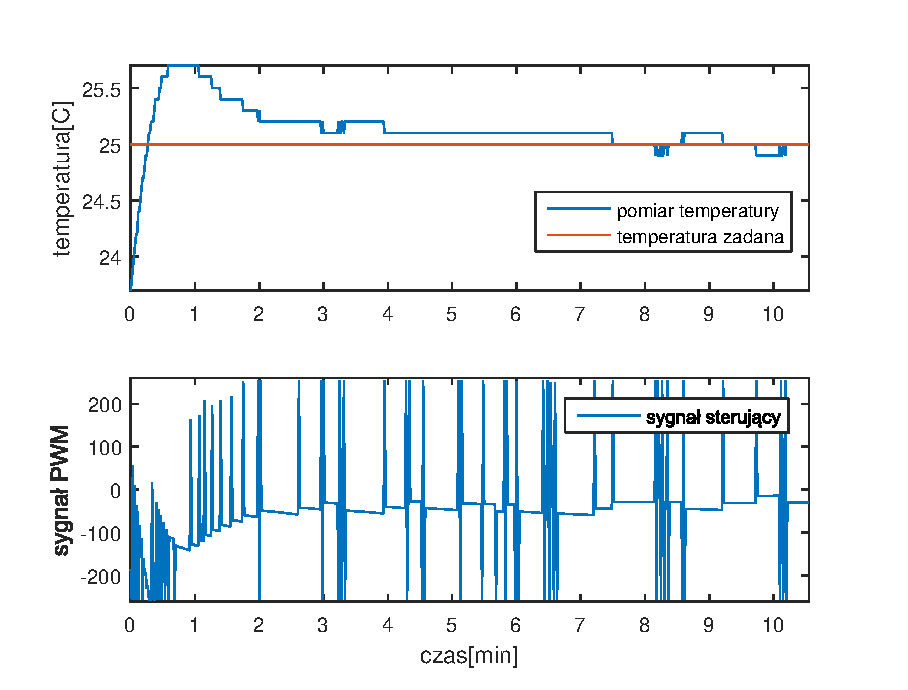
\includegraphics[scale=0.9]{pid25.eps}
	\caption{Regulacja dla $25^{\circ} C$ }
	\label{fig:pid25}
\end{figure}
\begin{figure}[H]
	\centering
	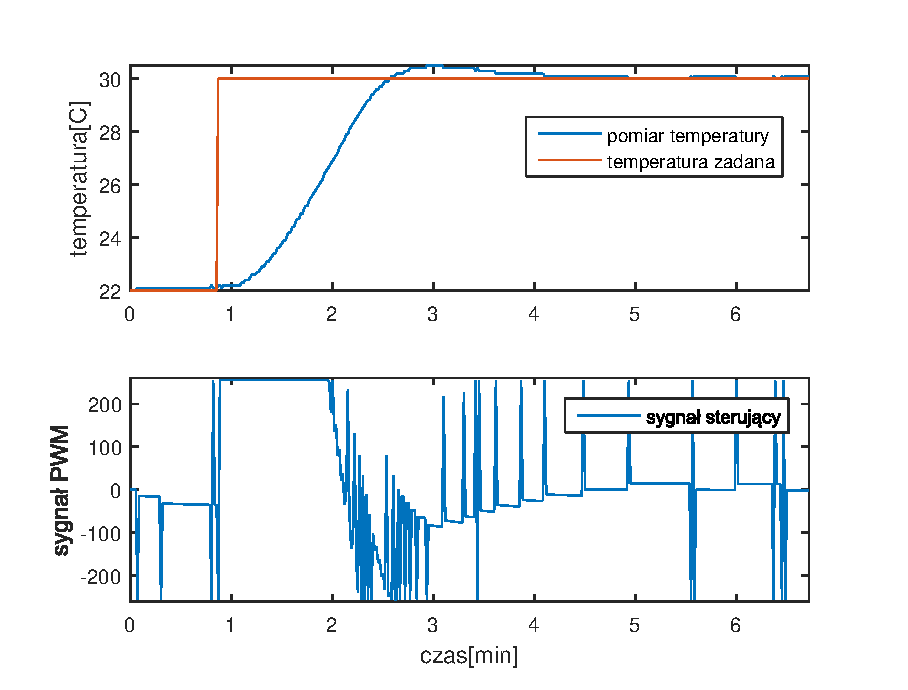
\includegraphics[scale=0.9]{pid30.eps}
	\caption{Regulacja dla $30^{\circ} C$ }
	\label{fig:pid30}
\end{figure}
\section{Aplikacja mobilna}
Podczas wykonywania pomiarów, nastawy oraz wartości zadane były przesyłane przez aplikację mobilną. W celu wygenerowania wykresów, do Arduino został podłączony komputer, nasłuchujący informacje przesyłane przez Arduino na porcie UART. Poniżej zamieszczono kilka zdjęć, wykonanych podczas regulacji temperatury za pomocą regulatora PID.
\begin{figure}[H]
	\centering
	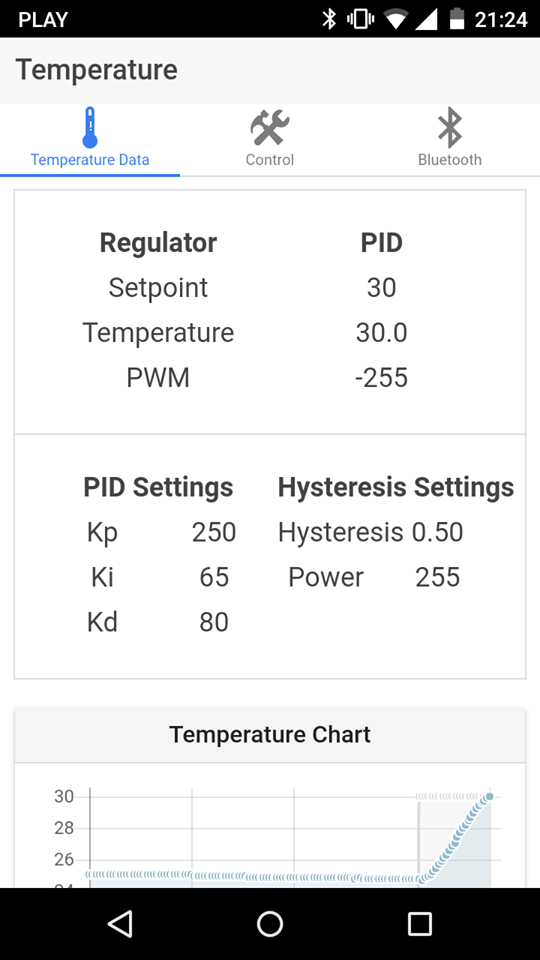
\includegraphics[scale=0.25]{testApki1.png}
	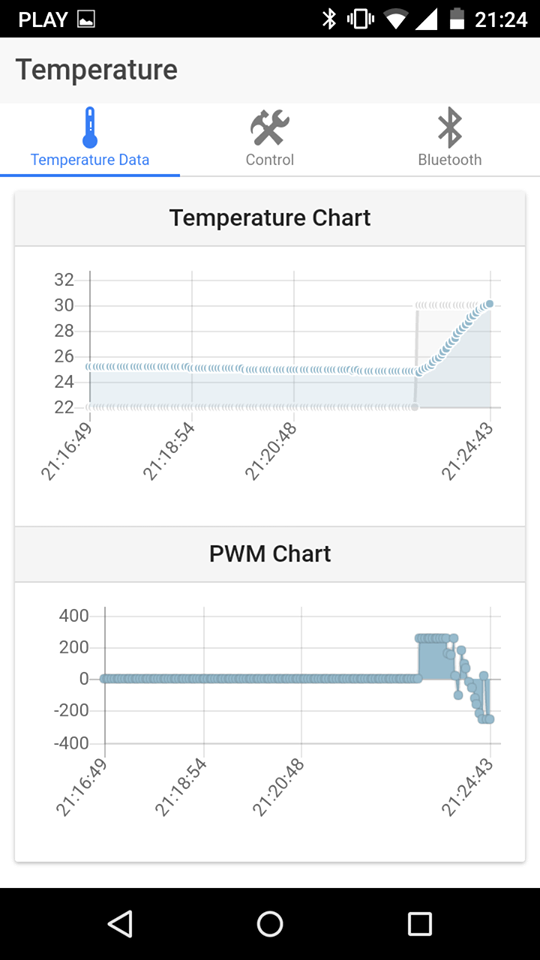
\includegraphics[scale=0.25]{testApki2.png}
	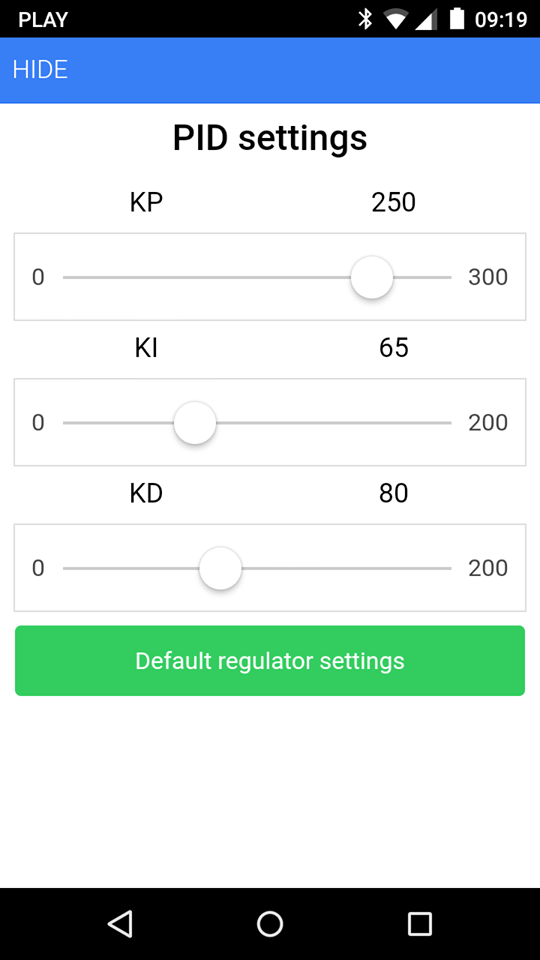
\includegraphics[scale=0.25]{apka4.png}
	\caption{Test działania aplikacji}
\end{figure}